\documentclass[NET,a4,12pt,ngerman]{netforms}

\usepackage[utf8]{inputenc}
\usepackage{tumcommon/tumlang}
\usepackage{tumcommon/tumcontact}
% \usepackage{scrpage2}

\documentclass[tikz]{standalone}

%
% This is a direct copy of the codes in section 2.9 of the package
% documentation (See page 45) https://mirrors.tuna.tsinghua.edu.cn/CTAN/graphics/pgf/contrib/pgfgantt/pgfgantt.pdf 
% except the color setting


\usepackage{pgfgantt}
\usepackage{xcolor}
\usepackage[utf8]{inputenc}

\definecolor{barblue}{RGB}{153,204,254}
\definecolor{groupblue}{RGB}{51,102,254}
\definecolor{linkred}{RGB}{165,0,33} 


\geometry{%
	top=10mm,
	bottom=10mm,
	left=25mm,
	right=25mm,
	headsep=1.5cm,
	includehead,
}
% /////////////////////////////////////////////////
% \documentclass{article}
\usepackage{graphicx}
\graphicspath{ {./images/} }


% Alle Konfigurationsbefehle sind optional. Fehlende Befehle fueheren einfach
% zu "blank forms".

% Typ der Arbeit/Einstellung. Gueltige Argumente sind:
% bachelor,master,diplom,idp,gr,hiwi,other
% Falls 'other' gewaehlt wird, kann als optionales Argument eine spezielle Art
% von Abschlussarbeit angegeben werden, z.B. \type[Sklave]{other}. Andernfalls
% wird 'Other' als Standardbeschreibung gesetzt.
\type{bachelor}

% Informationen ueber den Studenten. Sollte selbsterklaerend sein.
\anrede{Herr}
\nachname{nachname}
\vorname{vorname}
\matrikel{matrikel}
\sunhalle{sunaccount}
\semester{1}{SoSe\,2016}
\studientelefon{}{tel}
\heimattelefon{}{--}
\studienadresse{strasse}{plz stadt}
\heimatadresse[adresszusatz=,appartment=]{}{}
\mail{student@tum.de}

% Informationen ueber die Arbeit. Sollte selbsterklaerend sein.
\themensteller{\NEThead}
\beginn{04}{2016}
\endt{08}{2016}
\betreuer{Stephan G\"unther, Maurice Leclaire}
\title{English Title of My Thesis}{Englischer Titel Meiner Arbeit}
\studiengang{Informatik}


% Falls \type{hiwi} gesetzt wurde, wird die Taetigkeit auf dem Aufnahmeformular
% des Lehrstuhls angegeben.
\taetigkeit{test}



% \pagestyle{scrheadings}
% \clearscrheadfoot
% \chead{\TUMheader{1cm}}

\renewcommand{\maketitle}{%
	\begin{center}
% 		\textbf{\introductoryheadline}%
        \textbf{Antrittsvortrag zur Masterarbeit}\\
		\Large%
		\textbf{Efficient and Accurate Hop-by-Hop Capacity Estimation}%
	\end{center}

	\footnotesize%
	\hrule
	\vskip1ex
	\begin{tabular}{ll}
		\thenamelabel: &  \textbf{Bakar Andguladze}\\
		\theadvisorlabel: & \text{Simon Bauer, Benedikt Jaeger}\\
		\thesupervisorlabel: & \chairhead\\
		\thebeginlabel: & {01/2021}\\
		\theendlabel: & {07/2021}\\
	\end{tabular}
	\vskip1ex
	\hrule
	\vskip4ex
}

\linespread{1.2}
\setlength{\parskip}{.5\baselineskip}

\begin{document}
\maketitle

\subsection*{Topic}

This Master's Thesis shall implement a capacity estimation method for Hop-by-Hop measurements.
The intended field of application is, for instance, enhancing the performance of network, traffic analysis, network monitoring, etc.  Our main motivation is to improve the quality of the network and for that we require proper measurements of network capacity in order to, for instance, diagnose possible problems in it.

There are quite a few measurement tools available, such as, PPrate, Pathrate, Pathchar, etc. However the current State-of-the-Art methods have some significant flaws and limitations, such as: 
\begin{itemize}
    \item Active tools require considerable amount of probes and this might cause network overload\cite{BrzozaThesis} which might result in lost packets, queue delays, etc.\cite{AbutOverview}
    \item Passive tools analyze only ongoing traffic, therefore they're dependent on the traffic they observe. Also they require TCP server to respond
    Although they're widely used in practice and deliver reliable results, they're not enough to deliver all the desired information, such as the location of the narrow link, the exact path of the packets, etc.
    \item Trade-offs between intrusion and accuracy is hard to define.
\end{itemize}

Therefore our goal is to develop a new solution based on an active measurement technique that will employ the better parts of both passive and active tools, namely it will try to implement the least possible intrusion without compromising accuracy. Also it will be able to find the narrow link of the path by measuring the capacity of each hop in the network.
This new solution will be tested and evaluated by comparing it to the results of the existing capacity measurement tools.


The thesis is thematically related to the Bachelor's Thesis \emph{Implementation and Evaluation of Passive Capacity Estimation} \cite{BrzozaThesis} by Patryk Brzoza, but in contrast to Brzoza's passive approach our tool will be based on active measurement methodology. Moreover Brzoza's measurement tool was trying to find end-to-end capacity, while this thesis is concerned about measuring the capacity of each hop in the network and finding the narrow link. Hop-by-Hop measurement provides a better picture of the network and helps us take a look at the existing and possible issues more closely.
The thesis will go through the following research questions:
\begin{itemize}
    \item How to measure network capacity hop-by-hop?
    \item How to optimize the trade-off between accuracy and intrusiveness?
    \item How robust is the proposed solution?
    \item Are we able to locate the bottlenecks of the network?
\end{itemize}



\subsection*{Approach}
The thesis will be divided into two main parts:

The first part is the implementation of the tool. It will use active probing in order to generate the traffic to the routers and gather the received ICMP messages. Afterwards a passive measurement method will be applied to the gathered data. However, passive techniques are used for measuring end-to-end capacity and the main point of our approach is that we assume that each router of the network where packets pass is an endpoint. Hence, we basically measure End-to-End capacity of each hop. 
For example, on Figure 1, we will measure the capacity of C_1$ and assume it is the narrow link. Afterwards C_1$+C_2$ will be measured and checked if its capacity is smaller than the current narrow link. The measurement will continue to the following ones until it reaches the final endpoint.

\begin{figure}[h]
    \centering
    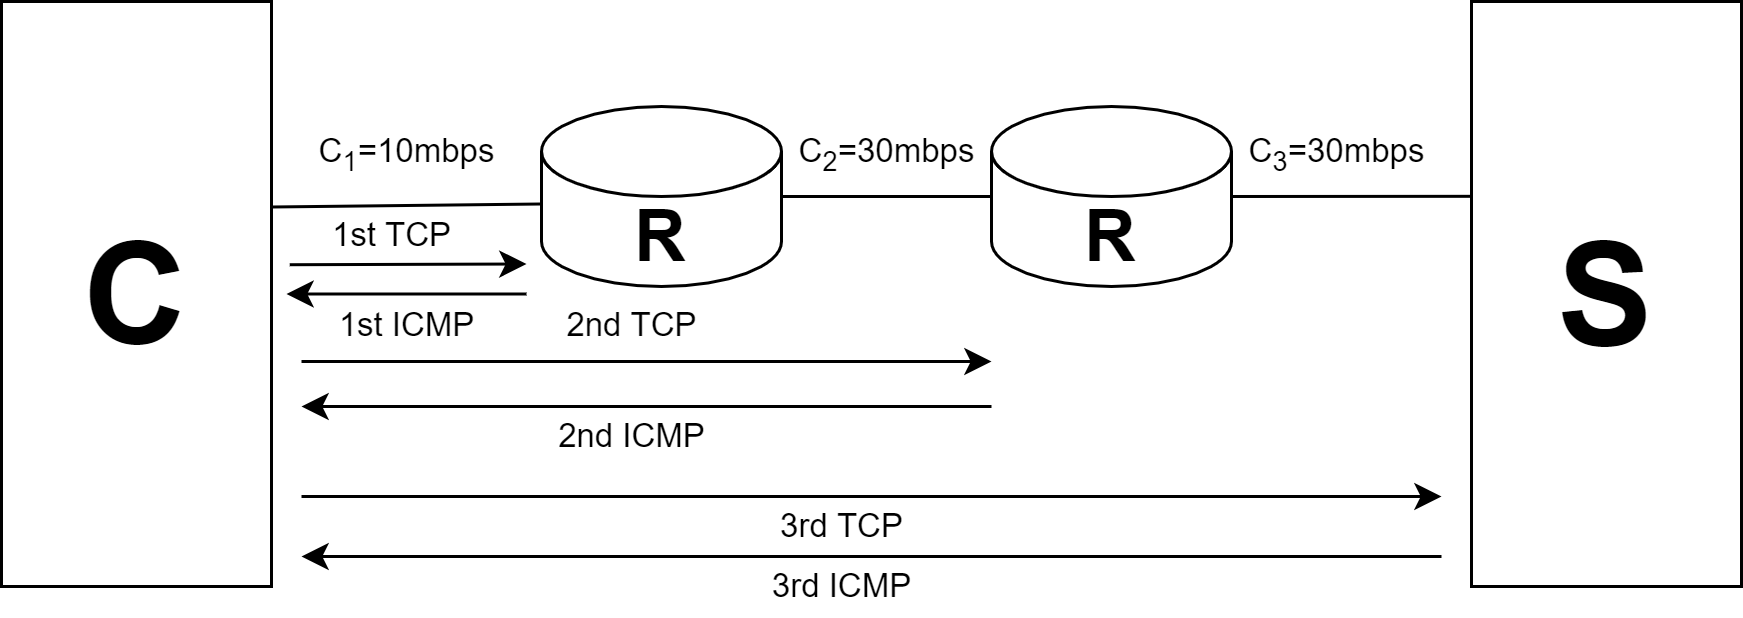
\includegraphics[scale=0.3]{images/NetworkDiag.png}
    \caption{Sample Network}
    \label{fig:mesh1}
\end{figure}


The second part of the thesis will be the evaluation. 
The first evaluation will be performed in the test environment using virtual network tool \textbf{\textit{mininet}}. For the maximum effectiveness various combinations of test parameters will be used. 


We will compare the new solution with the existing ones, such as, PPrate\cite{PPrate} and Brzoza's solution\cite{BrzozaThesis}. The different measurements will be conducted using the tools mentioned above and the results will be analyzed based on different test parameters, such as path lengths, cross traffic, capacities, delays and how these parameters influence the accuracy of measurements. Then these results will be compared to those of existing tools and methodologies, mainly the Passive Capacity Estimation by Brzoza \cite{BrzozaThesis}. 

The second evaluation will be conducted on a real network by taking additional factors into consideration, such as size of traffic at different times and hours. 

The measurement tool will be developed in Python and all the necessary operations will be performed on Ubuntu operating system.

The estimated timetable for this thesis can be seen below\colon

\begin{figure}[h]
    \centering
    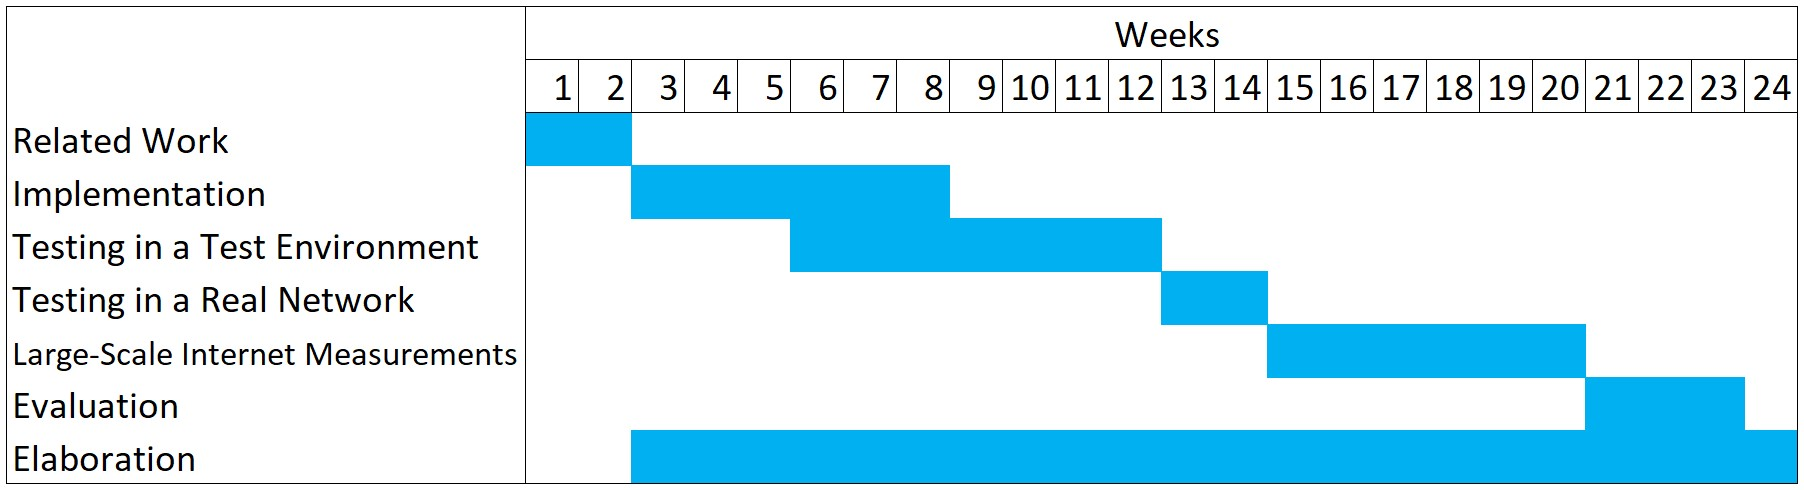
\includegraphics[scale=0.3]{images/GanttChart.jpg}
    \caption{Planned weekly schedule}
    \label{fig:mesh1}
\end{figure}



% \begin{ganttchart}[
%     \width=\linewidth,
%     y unit title=0.4cm,
%     y unit chart=0.5cm,
%     vgrid,
%     time slot format=isodate-yearmonth,
%     compress calendar,
%     title/.append style={draw=none, fill=barblue},
%     title label font=\sffamily\bfseries\color{white},
%     title label node/.append style={below=-1.6ex},
%     title left shift=.05,
%     title right shift=-.05,
%     title height=1,
%     bar/.append style={draw=none, fill=groupblue},
%     bar height=.6,
%     bar label font=\normalsize\color{black!50},
%     group right shift=0,
%     group top shift=.6,
%     group height=.3,
%     group peaks height=.2,
%     bar incomplete/.append style={fill=green}
%   ]{2010-09}{2011-12}
%   \gantttitlecalendar{year}\\
%   \ganttbar[
%     progress=100,
%     bar progress label font=\small\color{barblue},
%     bar progress label node/.append style={right=4pt},
%     bar label font=\normalsize\color{barblue},
%     name=pp
%   ]{Preliminary Project}{2010-09}{2010-12} \\
% \ganttset{progress label text={}, link/.style={black, -to}}
% \ganttgroup{Objective 1}{2011-01}{2011-12} \\
% \ganttbar[progress=4, name=T1A]{Task A}{2011-01}{2011-06} \\
% \ganttlinkedbar[progress=0]{Task B}{2011-07}{2011-12} \\
% \ganttgroup{Objective 2}{2011-01}{2011-12} \\
% \ganttbar[progress=15, name=T2A]{Task A}{2011-01}{2011-09} \\
% \ganttlinkedbar[progress=0]{Task B}{2011-10}{2011-12} \\
% \ganttgroup{Objective 3}{2011-05}{2011-08} \\
%   \ganttbar[progress=0]{Task A}{2011-05}{2011-08}
%   \ganttset{link/.style={green}}
%   \ganttlink[link mid=.4]{pp}{T1A}
%   \ganttlink[link mid=.159]{pp}{T2A}
% \end{ganttchart}


% \subsection*{Additional hardware requirements}
% \begin{itemize}
% 	\item 2 chassis for the USRPs \cite{chassiusrp}
% \end{itemize}

% \bibliographystyle{IEEEtran}
% \bibliography{IEEEabrv,lit}
\begin{thebibliography}{9}
\bibitem{PPrate} 
Taoufik En-Najjary, Guillaume Urvoy-Keller: PPrate: A Passive Capacity Estimation Tool. France, 2006

\bibitem{AbutOverview} 
Fatih Abut: Through the Diversity of Bandwidth-Related Metrics, Estimation Techniques and Tools An Overview. Adana, Turkey. 2018

\bibitem{BrzozaThesis} 
Patryk Brzoza: Implementation and Evaluation of Passive Capacity Estimation. 
Munich, 2018.

\bibitem{capest} 
Nicolas Kagami, et al.: CAPEST - Offloading Network Capacity and Available Bandwidth Estimation to Programmable Data Planes. Brazil, 2019

\bibitem{davrolis} 
Constantinos Dovrolis, et al. - Packet-Dispersion Techniques and a Capacity-Estimation Methodology. 2004

\bibitem{BrzozaGR}
Patryk Brzoza, et al.: Accuracy Optimization of Passive Capacity Estimation 

\bibitem{mininet}
R.L.S. De Oliveira, et.al. “Using Mininet for Emulation and Prototyping Software-Defined Networks" 2014
\end{thebibliography}

\end{document}
